\subsection{A New Conceptual Model for Mathematical VREs}\label{sec:tetrapod}
The probably most fundamental progress for a mathematical research environment is a new understanding of the aspects of virtual research environments reached via the intensive work with the semantics of VREs in \WPref{dksbases}.  We have codified the experiences in the OpenDreamKit project into a tetrapodal view on ``doing
mathematics'' -- i.e. the activity to be supported by a VRE.

We propose that all mathematical VREs need to support the following four main aspects at scale:
\begin{compactenum}[\em i\rm)]
\item \textbf{Inference}: deriving statements by \emph{deduction} (i.e.,
  proving), \emph{abduction} (i.e., conjecture formation from best
  explanations), and \emph{induction} (i.e., conjecture formation from examples).
\item \textbf{Computation}: algorithmic manipulation and simplification
  of mathematical expressions and other representations of
  mathematical objects.
\item \textbf{Tabulation}: generating, collecting, maintaining, and accessing
  collections of examples that suggest patterns and relations and allow testing
  of conjectures. 
\item \textbf{Narration}: bringing the results into a form that can be digested by humans,
  usually in mathematical documents like articles, books, or preprints, that expose the
  ideas in natural language but also in diagrams, tables, and simulations.
\end{compactenum} 

\begin{figure}[ht]\centering
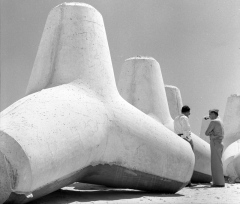
\includegraphics[width=5cm]{tetrapod}\qquad
\documentclass{standalone}
\usepackage{tikzinput}
\begin{document}
\providecommand\myscale{4.5}
\begin{tikzpicture}[scale=\myscale]
  \node (center) at (0,.15) {Organization};
  \node (left) at (.2,-.3) {Computation};
  \node (right) at (.4,0) {Tabulation};
  \node (back) at (-.5,0) {Inference};
  \node (up) at (0,.5) {Narration};

  \draw[very thick] (center) -- (left);
  \draw[very thick] (center) -- (right);
  \draw[very thick] (center) -- (back);
  \draw[very thick] (center) -- (up);
  \draw[dotted] (left) -- (right) -- (back) -- (left);
  \draw[dotted] (up) -- (left);
  \draw[dotted] (up) -- (right);
  \draw[dotted] (up) -- (back);
\end{tikzpicture}
\end{document}
%%% Local Variables: 
%%% mode: latex
%%% TeX-master: t
%%% End: 

\caption{Five Aspects of Math VREs, a Tetrapod Structure}\label{fig:tetrapod}
\end{figure}
Computer support exists for all of these four aspects of Big Math, e.g.,
\begin{compactenum}[\em i\rm)]
\item theorem provers like Isabelle, Coq, or Mizar;
\item computer algebra systems like GAP, SageMath, Maple, or Mathematica; and
\item mathematical data bases like the L-functions and Modular Forms Data 
Base (LMFDB)~\cite{Cremona:LMFDB16,lmfdb:on} and the Online Encyclopedia of
Integer Sequences (OEIS)~\cite{Sloane:OEIS};
\item online journals, mathematical information systems like zbMATH or MathSciNet,
  preprint servers like arXiv.org, or research-level help systems like MathOverflow.
\end{compactenum}
Humans can easily integrate these four aspects and do that for all mathematical developments, the corresponding integration in software systems is still a significant problem. It is our experience from the \pn project that one of the prerequisites is a \textbf{modular organization} of all four aspects in terms of a joint \textbf{mathematical ontology} -- the Math-in-the-Middle (MitM) ontology introduced in \WPref{dksbases} of the \pn project.

\def\hateq{\ensuremath{\widehat=}\xspace} Figure~\ref{fig:tetrapod} organizes these four aspects into a tetrapodal structure with the MitM ontology.  This model extends and refines he Data/Knowledge/Software model of the proposal by ``narration'' and ``organization'' aspects (Data (D) \hateq Tabulation, Knowledge (K) \hateq Inference, and Software (S) \hateq Computation). For details and a discussion in terms of ``big math'' developments like the classification of finite simple groups, consult~\cite{CarFarKohRab:bmobb19}.

The tetrapod model is consistent with the \pn structure and organization: the software aspect is mostly covered by \WPtref{hpc} and \WPtref{component-architecture} in \pn, where the latter develops the aspect of modular \textbf{organization} of the software. \WPtref{UI} covers the interaction between \textbf{Narration} and \textbf{Software} -- again, one of the innovations in the Jupyter framework concerns the modular \textbf{Organization} of software interfaces. \textbf{Inference} and \textbf{Tabulation} are covered in \WPtref{dksbases}.

We will now introduce three aspects that have been studied in detail in \pn in the last year and make up the technical bulk of this report in the sections after this one.  

%%% Local Variables:
%%% mode: latex
%%% mode: visual-line
%%% fill-column: 5000
%%% TeX-master: "report"
%%% End:

%  LocalWords:  WPref dksbases tetrapodal textbf emph Cremona:LMFDB16,lmfdb:on zbMATH organization centering includegraphics qquad hateq ensuremath widehat xspace CarFarKohRab:bmobb19 WPtref hpc WPtref WPtref Jupyter WPtref
